\setlength{\columnsep}{3pt}
\begin{flushleft}
	\paragraph{What is SUID?}
	\begin{itemize}
		\item SUID stands for \textbf{S}et \textbf{U}ser \textbf{ID}.
		\item \textbf{SUID can be applied only on command binaries}.
		\item \textbf{SUID is applicable only on user}.
		\item SUID allows user to run a \textbf{command binary} with the permissions of the \textbf{command binary owner} rather than the user who runs it.
		\item SUID is denoted as \textbf{"s"}, if user has execute permission.
		\begin{figure}[h!]
			\centering
			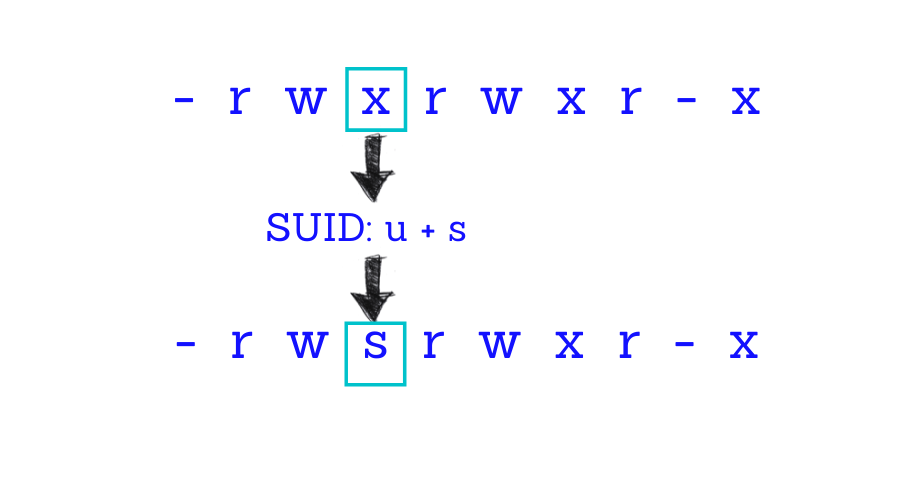
\includegraphics[scale=0.3]{content/chapter6/images/adv_perm1.png}
			\caption{SUID permission}
			\label{fig:combination_permission3}
		\end{figure}
		\item SUID is denoted as \textbf{"S"}, if no execute permission is applied for user.
		\begin{figure}[h!]
			\centering
			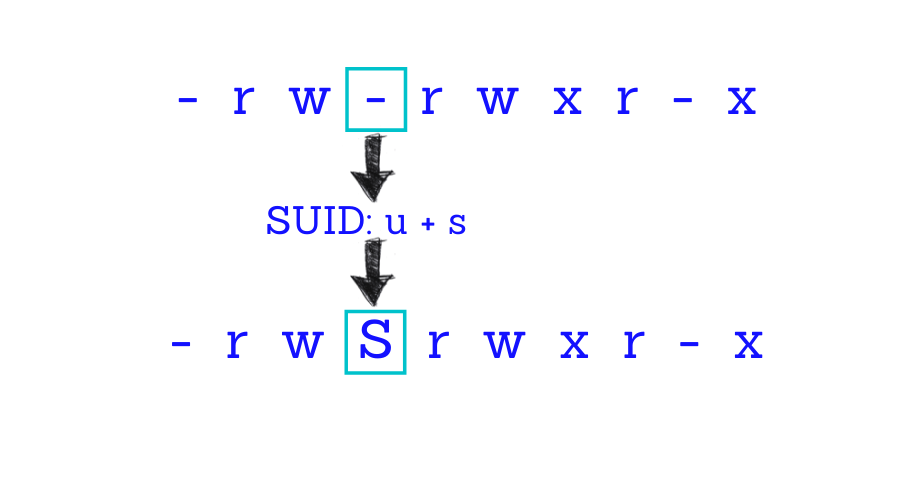
\includegraphics[scale=0.3]{content/chapter6/images/adv_perm2.png}
			\caption{SUID permission}
			\label{fig:combination_permission4}
		\end{figure}
		\item Octal representation of SUID permission is \textbf{"4"}.
	\end{itemize}
	\newpage
	\paragraph{Real world example for SUID}
	The \textbf{passwd} command has SUID applied on it.
	\bigskip
	\begin{tcolorbox}[breakable,notitle,boxrule=-0pt,colback=black,colframe=black]
		\color{green}
		\fontdimen2\font=1em
		\$ ls -ld /usr/bin/passwd
		\color{white}
		\newline
		\fontdimen2\font=0.5em
		-rwsr-xr-x 1 root root 68208 Jul 15  2021 /usr/bin/passwd
		\fontdimen2\font=4pt
	\end{tcolorbox}
	Explaination:
	\begin{itemize}
		\item The \textbf{passwd} command is used to change password.
		\item The command tries to edit files such as \textbf{/etc/passwd, /etc/shadow} etc. while changing the password.
		\item These files \textbf{can be accessed by root \& not local users}.
		\item The \textbf{SUID} permission allows local user to execute passwd command as root \& edit \textbf{/etc/passwd, /etc/shadow} files.
		\item Hence passwd command can be used by local user to change their own password.
	\end{itemize}
	
	\newpage
	
	\paragraph{How to apply SUID permission?}
	\begin{tcolorbox}[breakable,notitle,boxrule=0pt,colback=pink,colframe=pink]
		\color{black}
		\fontdimen2\font=1em
		Syntax: chmod u+s command\_binary
		\fontdimen2\font=4pt
	\end{tcolorbox}
	
	Let's take example of \textbf{fdisk} command. 
	\newline
	The \textbf{fdisk command cannot be executed by normal user and is owned by root user}. Is there a way to allow local user execute \textbf{fdisk} commnd?
	\newline
	\textbf{Solution}: 
	\begin{itemize}
		\item Apply SUID on the \textbf{fdisk} command binary.
		\item 	SUID can be set in two ways:
		\bigskip
		\begin{tcolorbox}[breakable,notitle,boxrule=-0pt,colback=black,colframe=black]
			\color{green}
			\fontdimen2\font=1em
			\# chmod u+s  /usr/sbin/fdisk
			\newline
			or
			\newline
			\# chmod 4750 /usr/sbin/fdisk
			\newline
			\newline
			\# ls -ld /usr/sbin/fdisk
			\newline
			\color{white}
			-rwsr-xr-x 1 root root 153880 Jul 21  2020 /usr/sbin/fdisk
			\fontdimen2\font=4pt
		\end{tcolorbox}
		\item Check if \textbf{normal user jack} is able to execute \textbf{fdisk} command:
		\begin{tcolorbox}[breakable,notitle,boxrule=-0pt,colback=black,colframe=black]
			\color{green}
			\fontdimen2\font=1em
			jack@lavatech:~\$ fdisk -l
			\fontdimen2\font=4pt
		\end{tcolorbox}
	\end{itemize}
	\paragraph{How to remove SUID permission?}
	\bigskip
	\begin{tcolorbox}[breakable,notitle,boxrule=0pt,colback=pink,colframe=pink]
		\color{black}
		\fontdimen2\font=1em
		Syntax: chmod u-s command\_binary
		\fontdimen2\font=4pt
	\end{tcolorbox}
	Eg:
	\begin{tcolorbox}[breakable,notitle,boxrule=-0pt,colback=black,colframe=black]
		\color{green}
		\fontdimen2\font=1em
		\# chmod u-s  /usr/sbin/fdisk
		\newline
		\color{white}
		OR
		\color{green}
		\newline
		\# chmod 0750 /usr/sbin/fdisk
		\fontdimen2\font=4pt
	\end{tcolorbox}

	
\end{flushleft}

\newpage

